\subsection*{Hypothesis 1}

Reviews with longer text have higher helpfulness ratings.\\
\noindent
\textbf{Metric:} Correlation coefficient (e.g., Pearson's correlation) between review length and helpfulness score.\\
\noindent
\textbf{Missing Values:}
\begin{itemize}
    \item \textit{`review/text`:} remove the entire sample
    \item \textit{`review/helpfulness`:} remove the entire sample
\end{itemize}
\noindent
\textbf{Data Transformation:}
\begin{itemize}
    \item \textit{`review/text`:} Count the number of words in each review removing punctuation and stopwords.
    \item \textit{`review/helpfulness`:} $helpfulness = \frac{x}{y} \sqrt(y)$
\end{itemize}\vspace{0.5cm}
\noindent
\textbf{Description and Results}
The data cleaning and 'review/helpfulness' transformation process was performed using the \textit{`pymongo`} library to exploit the 
MongoDB efficiency. Specifically, we defined a pipeline to perform the needed operations. As regards the 
'review/text' transformation, we used the \textit{`nltk`} library to tokenize the text, remove punctuation, stopwords and eventually
count the number of words.\\
The correlation coefficient between the two variables is $0.3313$ with a p-value $<0.05$, indicating a statistically significant correlation.\\
A graphical confirmation is provided by Figure \ref{fig:h1_boxplot}. Indeed there is a positive correlation until around 400 words, after which the
boxplot stabilizes. Thereby, we decided to analyze the correlation within the review length groups. As a results (Table \ref{corr_groups}) we got that the correlation is
positive and statistically significant for the reviews with length between 0 and 400 words, while it becomes negative and statistically significant
for the reviews with length greater than 750 words. As regards the reviews in the middle (i.e. between 400 and 750 words), the correlation is negligible.\\
\textbf{Conclusion:} The hypothesis is confirmed, but the correlation is not very strong and changes depending on the review length.\\

\begin{figure}[H]
    \centering
    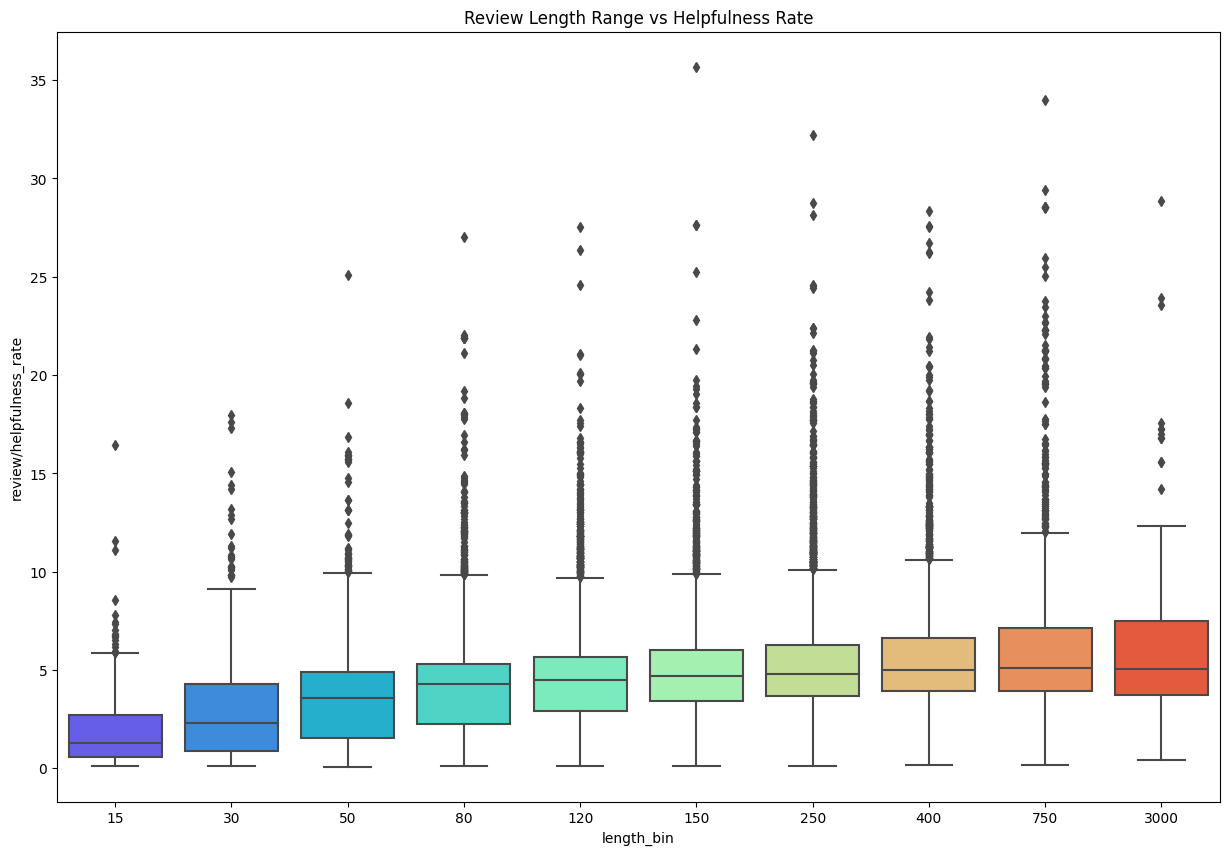
\includegraphics[width=0.5\textwidth]{./figures/h1_scatter.png}
    \caption{Correlation between review length and helpfulness score for different review length groups}
    \label{fig:h1_scatter}
\end{figure}

\begin{table}[H]
    \centering
    \caption{Correlation Coefficients and P-values for Different Groups}
    \begin{tabular}{|c|c|c|}
    \hline
    Group Number & Correlation Coefficient & P-value \\
    \hline
    400 & 0.2216 & 0.0000 \\
    \hline
    750 & -0.0188 & 0.2585 \\
    \hline
    3000 & -0.1418 & 0.0065 \\
    \hline
    \end{tabular}
    \end{table}
\label{corr_groups}
